\section{Hair}
To simulate hair, angular springs are used. Our implementation of the angular spring is not directly based on a behaviour function, but instead combines the usage of damped springs and rod constraints such that a triplet of particles are pulled so that their subtending angle approaches some rest angle. In figure \ref{fig:Angular Spring}, the structure in which the springs and rods are configured is shown. \\
\begin{figure}[h]
    \centering
    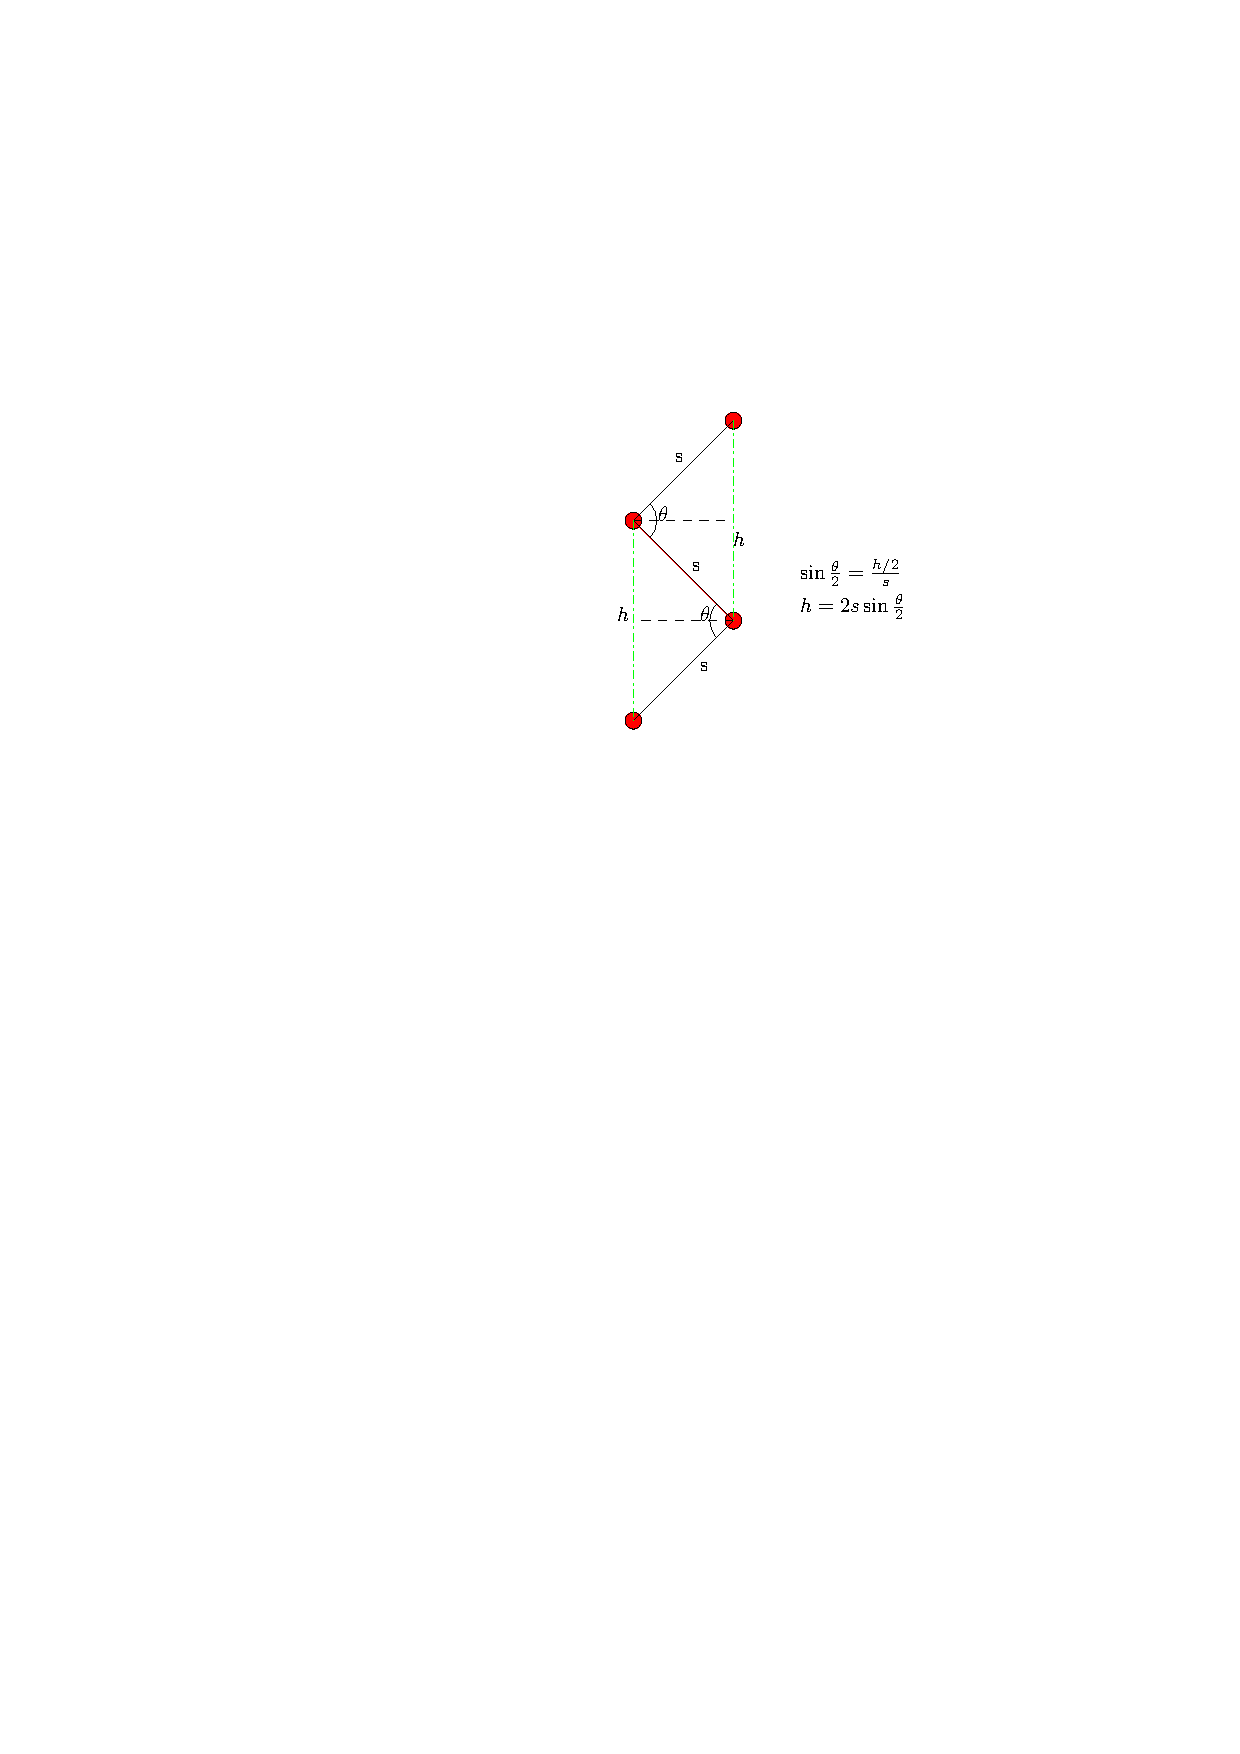
\includegraphics[width=0.4\textwidth]{hair}
    \caption{Representation angular spring}
    \label{fig:Angular Spring}
\end{figure}
The green dotted dashed lines in the figure are representing springs with rest length $h$ and the black solid lines are representing rod constraints of length $s$. The calculations to calculate the rest length is also given for some rest angle $\theta$. In this way, the rods will ensure that each hair segments is of constant length and the damped springs will pull or repel the first and the last particle of the triplet until the rest angle is reached.\\
By using the last particle of the tripled as the first particle of a new triplet, it is possible to create a chain which can represent a string of hair. 